% APS-style scientific article
% Compile with: pdflatex main.tex (requires revtex4-2)
\documentclass[aps,prx,reprint,showpacs,showkeys,floatfix]{revtex4-2}

\usepackage{amsmath,amssymb}
\usepackage{braket}
\usepackage{graphicx}
\usepackage{dcolumn}
\usepackage{bm}
\usepackage{hyperref}

\begin{document}

\title{CHEM 5260 Midterm Project \\
A preliminary theoretical and numerical investigation on quantum relaxation}

\author{Wenxiang Ying}
\email{wying3@sas.upenn.edu}
\affiliation{Department of Chemistry, University of Pennsylvania,
             Philadelphia, Pennsylvania 19104, USA}

\date{\today}

\begin{abstract}
We present a combined analytical and numerical study of quantum relaxation
dynamics in two finite-dimensional doorway-state models.  Model~A consists
of a single doorway state $\ket{1}$ coupled to a discrete manifold of bath
states $\{\ket{k}\}$, while Model~B adds an upstream state $\ket{0}$ so
that population flows sequentially as $\ket{0}\to\ket{1}\to\{\ket{k}\}$.
The analytical treatment is based on Green's functions and self-energies
under the wide-band approximation, while the exact finite-dimensional
dynamics is obtained independently from the full Hermitian Hamiltonian by
exact diagonalization.
For Model~A the theory recovers the Fermi's-golden-rule prediction
$P_1(t)=e^{-\Gamma t}$ with $\Gamma=2\pi|V|^2\rho$, and the numerics show
that this exponential regime is realized when $\rho^{-1}\lesssim\Gamma\ll
\Delta E$, while finite bath size, narrow bandwidth, or strong coupling
produce non-Markovian oscillations and Poincar\'e recurrences.  For Model~B,
the same wide-band reduction assumes that the doorway state $\ket{1}$
undergoes Markovian exponential decay with rate $\Gamma$, so that the pair
$\{\ket{0},\ket{1}\}$ becomes a damped two-level system with overdamped,
critically damped, and underdamped regimes separated by the threshold
$V_{01}=\Gamma/4$.  Numerical scans over $N$, $\Delta E$, $V_{1k}$,
$V_{01}$, and the detuning $E_0-E_1$ quantitatively confirm the analytical
predictions, including the Lorentzian resonance profile and the crossover
from monotonic transfer to damped Rabi oscillations.  Random-sign couplings
are found to be gauge-equivalent to uniform couplings, whereas
Gaussian-distributed couplings preserve the mean decay trend but broaden the
ensemble of trajectories.
\end{abstract}

\keywords{quantum relaxation, doorway-state model, Fermi's golden rule,
wide-band approximation, damped two-level system, Poincar\'e recurrence}

\maketitle
\tableofcontents

%-----------------------------------------------------------------------
\section{Introduction}
%-----------------------------------------------------------------------

Quantum relaxation is a fundamental phenomenon in chemical physics that
underlies processes ranging from intramolecular vibrational energy
redistribution and electronic energy transfer to non-radiative decay and
photochemical reactions~\cite{Nitzan}.  In a minimal doorway-state picture,
an initially populated ``bright'' state is coupled to a dense manifold of
background states, and population leaks out on a timescale governed by the
manifold density of states and the coupling matrix elements.

The analytical theory of such processes, developed via Green's function and
self-energy methods~\cite{Nitzan,Weiss}, predicts that the survival probability of the doorway
state decays exponentially in time when the manifold is sufficiently broad
and dense to be treated as a quasi-continuum.  The exponential decay rate is
given by Fermi's golden rule (FGR):
\begin{equation}
    \Gamma = 2\pi|V|^2\rho,
    \label{eq:FGR}
\end{equation}
where $\rho$ is the density of states of the bath manifold and $V$ is a
characteristic coupling matrix element; throughout this paper we work in
units where $\hbar=1$.  This result rests on the
\emph{wide-band approximation}: the resonance width $\Gamma$ must be small
relative to the total bandwidth $\Delta E$ of the manifold, while remaining
large compared to the discrete level spacing $\rho^{-1}$:
\begin{equation}
    \rho^{-1} \lesssim \Gamma \ll \Delta E.
    \label{eq:wideband}
\end{equation}
When these inequalities are violated the dynamics can deviate markedly from
exponential, exhibiting quantum revivals, persistent oscillations, or
incomplete relaxation.  In other words, the irreversible Markovian decay
predicted by FGR is not a generic property of a finite bath, but a specific
limit that must be demonstrated.

In any finite numerical simulation, however, the manifold is discrete and
bounded, so the continuum picture can only emerge as an approximation over a
finite time window.  Understanding when and how that approximation breaks
down is therefore essential.

The present work addresses these questions through a combined analytical and
numerical study of two finite-dimensional model Hamiltonians.  Model~A is
the minimal doorway-state problem: a single state $\ket{1}$ coupled to a
bath manifold $\{\ket{k}\}$.  Model~B extends this construction by adding an
upstream state $\ket{0}$ coupled only to $\ket{1}$, so that the population
flow proceeds sequentially: $\ket{0}\to\ket{1}\to\{\ket{k}\}$.

For Model~A, Green's-function and self-energy methods~\cite{Nitzan,Weiss}
recover the standard wide-band result $P_1(t)=e^{-\Gamma t}$.  For Model~B,
the same wide-band
approximation implies that the doorway state $\ket{1}$ decays Markovianly
with rate $\Gamma$, so that the remaining pair $\{\ket{0},\ket{1}\}$ forms
an effective damped two-level system, i.e. a damped two-state Rabi
problem~\cite{CohenTannoudji1997}.  This yields a clear analytical
classification of the dynamics: overdamped for $V_{01}<\Gamma/4$, critical
at $V_{01}=\Gamma/4$, and underdamped for $V_{01}>\Gamma/4$.  Detuning
$E_0-E_1$ then enters as a resonance parameter that suppresses the
upstream-to-doorway transfer through a Breit--Wigner / Lorentzian line shape.

The numerical part of the work is based on exact diagonalization of the full
finite Hamiltonian, with no time-discretization or perturbative approximation.
By varying $N$, $\Delta E$, $V_{1k}$, $V_{01}$, and $E_0-E_1$, we test the
analytical predictions against the exact dynamics, identify the boundaries of
the wide-band regime, and compare uniform, random-sign, and Gaussian bath
couplings.

The central questions addressed here are: (i) under what conditions does a
finite discrete bath reproduce the exponential relaxation predicted by
Fermi's golden rule? (ii) how does breakdown of the wide-band approximation
manifest in finite systems? and (iii) how does the addition of an upstream
state generate distinct overdamped, critical, and underdamped regimes?

%-----------------------------------------------------------------------
\section{Model Hamiltonians and Methods}
\label{sec:models}
%-----------------------------------------------------------------------

\subsection{Model Hamiltonian}

\subsubsection{Model A}

The Hilbert space of Model~A is spanned by the orthonormal basis
$\{\ket{1}, \ket{k_1}, \ket{k_2}, \ldots, \ket{k_N}\}$.
The full Hamiltonian is
\begin{equation}
    \hat{H}_A = E_1\ket{1}\!\bra{1}
              + \sum_{k=1}^{N} E_k\ket{k}\!\bra{k}
              + \sum_{k=1}^{N}\bigl(V_{1k}\ket{1}\!\bra{k}
                                  + V_{k1}\ket{k}\!\bra{1}\bigr),
    \label{eq:HA}
\end{equation}
where $E_1$ is the energy of the doorway state and $E_k$ are the energies of
the bath levels.  All couplings are taken real so that $V_{k1}=V_{1k}$.
The bath energies are distributed uniformly over an interval of width
$\Delta E$ centred on $E_1$,
\begin{equation}
    E_k \in \Bigl[E_1 - \tfrac{\Delta E}{2},\; E_1 + \tfrac{\Delta E}{2}\Bigr],
    \label{eq:Ek}
\end{equation}
giving a continuum density of states $\rho = N/\Delta E$.
For the uniformly spaced numerical grids used below, the exact nearest-neighbour
spacing is $\Delta\omega = \Delta E/(N-1)$, so that in the large-$N$ limit
one has $\rho^{-1}\approx \Delta E/N \approx \Delta\omega$.  Without loss of
generality we set $E_1 = 0$.

The system is initialized in the doorway state, $\ket{\psi(0)} = \ket{1}$,
and the principal observable is the survival probability
\begin{equation}
    P_1(t) = |\braket{1|\psi(t)}|^2.
    \label{eq:P1}
\end{equation}
We also monitor the total bath population
$P_K(t) = \sum_{k=1}^{N}|\braket{k|\psi(t)}|^2 = 1 - P_1(t)$.

\subsubsection{Model B}

Model~B introduces an additional state $\ket{0}$ that is coupled only to
the doorway state $\ket{1}$, with no direct coupling to the bath.
The Hilbert space is thus $\{\ket{0}, \ket{1}, \ket{k_1}, \ldots,
\ket{k_N}\}$ and the Hamiltonian is
\begin{align}
    \hat{H}_B &= E_0\ket{0}\!\bra{0} + E_1\ket{1}\!\bra{1}
               + V_{01}\ket{0}\!\bra{1} + V_{10}\ket{1}\!\bra{0}
               \notag\\
              &\quad + \sum_{k=1}^{N} E_k\ket{k}\!\bra{k}
               + \sum_{k=1}^{N}\bigl(V_{1k}\ket{1}\!\bra{k}
                                   + V_{k1}\ket{k}\!\bra{1}\bigr).
    \label{eq:HB}
\end{align}
The total number of levels is $N+2$ and the initial condition is
$\ket{\psi(0)} = \ket{0}$.  The observables are
\begin{align}
    P_0(t) &= |\braket{0|\psi(t)}|^2, \\
    P_1(t) &= |\braket{1|\psi(t)}|^2, \\
    P_K(t) &= \sum_{k=1}^{N}|\braket{k|\psi(t)}|^2.
    \label{eq:P_B}
\end{align}

The energy-level structures of both models are illustrated in Fig.~\ref{fig:models}.

\begin{figure}[htbp]
    \centering
    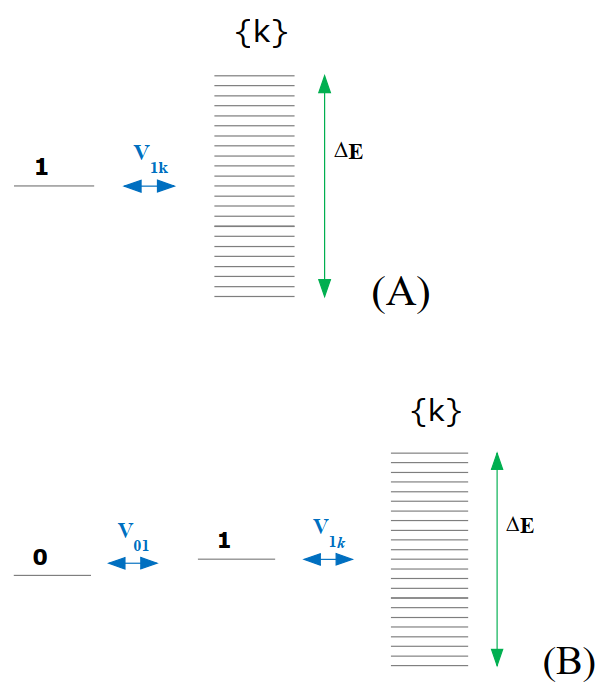
\includegraphics[width=1.0\linewidth]{Figure1.png}
    \caption{Energy-level diagrams for (A) Model~A, in which the doorway state
    $\ket{1}$ is coupled directly to the bath manifold $\{\ket{k}\}$ with matrix
    elements $V_{1k}$; and (B) Model~B, in which the upstream state $\ket{0}$
    is first coupled to $\ket{1}$ via $V_{01}$, and $\ket{1}$ subsequently
    couples to the manifold via $V_{1k}$.}
    \label{fig:models}
\end{figure}

\subsubsection{Coupling schemes}

Three coupling schemes are compared throughout.
\begin{enumerate}
    \item \emph{Uniform couplings}: all matrix elements equal,
          $V_{1k} = V$ for $k = 1,\ldots,N$.
    \item \emph{Random-sign couplings}: $V_{1k} = \pm V$ with equal probability,
          so that $\langle V_{1k}\rangle = 0$ and
          $\langle V_{1k}^2\rangle^{1/2} = V$.
    \item \emph{Gaussian couplings}: $V_{1k}\overset{\mathrm{i.i.d.}}{\sim}
          \mathcal{N}(0,V^2)$, so that $\langle V_{1k}\rangle = 0$ and
          $\langle V_{1k}^2\rangle^{1/2} = V$.
\end{enumerate}
Throughout, we denote the root-mean-square doorway--bath coupling by
\begin{equation*}
    V_{\mathrm{rms}} \equiv \langle V_{1k}^2 \rangle^{1/2},
\end{equation*}
so that $V_{\mathrm{rms}}=V$ for all three schemes above.  Whenever a
single characteristic coupling scale is needed analytically, we write
$V \equiv V_{\mathrm{rms}}$.

\subsection{Time-dependent Schr\"{o}dinger equation and exact diagonalization}
\label{sec:TDSE}

Since both Hamiltonians are represented by finite Hermitian matrices of
dimension $(N+1)\times(N+1)$ (Model~A) or $(N+2)\times(N+2)$ (Model~B),
the dynamics is governed by the time-dependent Schr\"{o}dinger equation
(TDSE),
\begin{equation}
    i\hbar\frac{d}{dt}\ket{\psi(t)} = \hat{H}\ket{\psi(t)},
    \label{eq:TDSE}
\end{equation}
whose formal solution is $\ket{\psi(t)}=e^{-i\hat{H}t/\hbar}\ket{\psi(0)}$.
Expanding in the energy eigenbasis $\hat{H}\ket{j}=E_j\ket{j}$,
\begin{equation}
    \ket{\psi(t)} = \sum_j e^{-iE_j t}\ket{j}\braket{j|\psi(0)},
    \label{eq:psit}
\end{equation}
where $\{E_j,\ket{j}\}$ are the eigenvalues and eigenvectors of $H$.
Numerically this spectral decomposition is obtained via the full
diagonalization $H = UDU^\dagger$, which gives
$e^{-iHt} = Ue^{-iDt}U^\dagger$.
This approach is exact within machine precision and avoids all time-stepping
errors.  We work in units where $\hbar = 1$ throughout, and all parameters
are reported in consistent dimensionless units.  Typical system sizes range
from $N = 50$ to $N = 200$ bath levels; convergence with respect to $N$ is
checked explicitly.

\subsection{Green's function treatment and the wide-band approximation}
\label{sec:GF}

The analytical benchmark for both models is obtained by combining the
retarded Green's function with the wide-band approximation~\cite{Nitzan,Weiss}.  For Model~A
this leads directly to Fermi's-golden-rule exponential decay.  For
Model~B, after the same wide-band reduction of the bath, the remaining
dynamics is that of a damped two-level system formed by the pair
$\{\ket{0},\ket{1}\}$.

\subsubsection{Model A: Green's function treatment under the wide-band approximation}

{\bf Equations of motion for the amplitudes}. Projecting the TDSE onto the basis states of Model~A and writing
$c_1(t)=\braket{1|\psi(t)}$ and $c_k(t)=\braket{k|\psi(t)}$, the
coupled amplitude equations are ($\hbar=1$)
\begin{align}
    i\dot{c}_1 &= E_1 c_1 + \sum_k V_{1k}\,c_k, \label{eq:c1dot}\\
    i\dot{c}_k &= E_k c_k + V_{k1}\,c_1. \label{eq:ckdot}
\end{align}
Formally integrating Eq.~\eqref{eq:ckdot} with $c_k(0)=0$ and substituting
back into Eq.~\eqref{eq:c1dot} yields an integro-differential equation for
$c_1(t)$, whose Laplace transform is most naturally analysed via the Green's
function.

{\bf Dyson equation and the self-energy}. The retarded Green's operator $\hat{G}(E)$ is defined as
\begin{equation}
    \hat{G}(E) = \lim_{\eta\to 0^+}(E - \hat{H} + i\eta)^{-1},
    \label{eq:Gret}
\end{equation}
and the survival amplitude is recovered by the inverse Fourier transform
\begin{equation}
    c_1(t) = \int_{-\infty}^{\infty}\frac{dE}{2\pi i}\,
             e^{-iEt}\,G_{11}(E), \qquad
    G_{11}(E) \equiv \braket{1|\hat{G}(E)|1}.
    \label{eq:c1_GF}
\end{equation}
Projecting the resolvent identity $(E-\hat{H})\hat{G}=\hat{1}$ onto
$\ket{1}$ and onto each $\ket{k}$ gives
\begin{equation}
    G_{k1}(E) = \frac{V_{k1}}{E - E_k + i\eta}\,G_{11}(E),
\end{equation}
and back-substituting yields the Dyson equation
\begin{equation}
    G_{11}(E) = \frac{1}{E - E_1 - \Sigma(E)},
    \label{eq:Dyson}
\end{equation}
where the self-energy is
\begin{equation}
    \Sigma(E) = \sum_{k=1}^{N}\frac{|V_{1k}|^2}{E - E_k + i\eta}.
    \label{eq:SelfEnergy}
\end{equation}

{\bf Wide-band approximation and exponential decay}. In the continuum limit Eq.~\eqref{eq:SelfEnergy} becomes an integral over
the bath density of states $\rho(\varepsilon)$:
\begin{equation}
    \Sigma(E) \to \int_{-\infty}^{\infty}d\varepsilon\,
                  \frac{|V(\varepsilon)|^2\rho(\varepsilon)}{E-\varepsilon+i\eta}.
    \label{eq:SigmaCont}
\end{equation}
Applying the Sokhotski--Plemelj identity
$\lim_{\eta\to 0^+}(x+i\eta)^{-1} = \mathcal{P}(1/x) - i\pi\delta(x)$
decomposes $\Sigma = \Delta(E) - \tfrac{i}{2}\Gamma(E)$ with the
energy-dependent decay rate
\begin{equation}
    \Gamma(E) = 2\pi|V(E)|^2\rho(E).
    \label{eq:GammaE}
\end{equation}
The \emph{wide-band approximation} (WBA) assumes
$|V(\varepsilon)|^2\rho(\varepsilon)\approx|V|^2\rho=\mathrm{const}$
across the resonance width, which holds when $\Gamma\ll\Delta E$ and $E_1$
lies well away from the band edges.  The energy shift $\Delta$ then vanishes
by symmetry and the self-energy reduces to a pure imaginary constant,
\begin{equation}
    \Sigma(E) \approx -\frac{i\Gamma}{2}, \qquad
    \Gamma = 2\pi|V|^2\rho.
    \label{eq:WBA}
\end{equation}
The Green's function $G_{11}(E)$~\eqref{eq:Dyson} becomes a Lorentzian pole,
\begin{equation}
    G_{11}(E) \approx \frac{1}{E - E_1 + i\Gamma/2},
    \label{eq:GLorentz}
\end{equation}
of half-width $\Gamma/2$ centered at $E_1$.  Evaluating the inverse
transform~\eqref{eq:c1_GF} by closing the contour in the lower half-plane
($t>0$) and picking up the single pole at $E=E_1-i\Gamma/2$,
\begin{equation}
    c_1(t) = e^{-iE_1 t}\,e^{-\Gamma t/2},
    \label{eq:c1_exp}
\end{equation}
so that the survival probability decays exponentially,
\begin{equation}
    P_1(t) = |c_1(t)|^2 = e^{-\Gamma t},
    \qquad \Gamma = 2\pi|V|^2\rho,
    \label{eq:FGR_pred}
\end{equation}
in agreement with Fermi's golden rule~\eqref{eq:FGR}.  The validity
conditions are exactly those of Eq.~\eqref{eq:wideband}; violations of
either bound lead to deviations from exponential behavior explored
numerically in the next section.

\subsubsection{Model B: damped two-level dynamics under the wide-band approximation}

For Model~B the bath still couples only through the doorway state
$\ket{1}$, so the same wide-band self-energy can be used after projecting
onto the two-dimensional subspace $\{\ket{0},\ket{1}\}$.  The bath degrees
of freedom are integrated out exactly as in Model~A, yielding the effective
non-Hermitian Hamiltonian
\begin{equation}
    H_{\mathrm{eff}}^{(B)} =
    \begin{pmatrix}
        E_0 & V_{01} \\
        V_{01} & E_1 - i\Gamma/2
    \end{pmatrix},
    \qquad
    \Gamma = 2\pi |V_{1k}|^2\rho.
    \label{eq:HeffB}
\end{equation}
The crucial assumption here is the \emph{wide-band approximation}: the bath
seen by $\ket{1}$ is taken to be sufficiently broad and dense that
$\Sigma(E)\approx -i\Gamma/2$ is energy independent, so the isolated doorway
state would decay Markovianly as $c_1(t)\propto e^{-iE_1 t}e^{-\Gamma t/2}$.
Only under this assumption can Model~B be reduced to an ordinary damped
two-level (Rabi) problem~\cite{CohenTannoudji1997}.  Equivalently, the amplitudes
$c_0(t)$ and $c_1(t)$ obey
\begin{align}
    i\dot{c}_0 &= E_0 c_0 + V_{01}c_1, \\
    i\dot{c}_1 &= V_{01}c_0 + \left(E_1 - i\frac{\Gamma}{2}\right)c_1.
    \label{eq:modelB_WBA_amp}
\end{align}

The complex normal-mode energies are obtained from the characteristic
equation of $H_{\mathrm{eff}}^{(B)}$:
\begin{equation}
    E_{\pm} =
    \frac{E_0 + E_1 - i\Gamma/2}{2}
    \pm
    \frac{1}{2}\sqrt{\left(E_0-E_1+i\Gamma/2\right)^2 + 4V_{01}^2},
    \label{eq:EpmB}
\end{equation}
which govern the exact WBA dynamics of the amplitudes $c_0(t)$ and $c_1(t)$.
At finite detuning $\Delta_{01}=E_0-E_1$, these poles interpolate between
coherent two-level oscillations and irreversible decay into the continuum.
If the wide-band approximation fails, the decay of $\ket{1}$ is no longer
strictly Markovian and the simple damping classification below ceases to be
quantitatively valid.

The analytical treatment above relies on two linked assumptions of the
wide-band approximation.  First, the bath density of states and coupling
strength must vary only slowly across the resonance width, so that the
self-energy may be treated as effectively energy independent.  Second, the
bath must be sufficiently dense on the timescale of the decay that it can
be treated as effectively continuous, i.e.\ $\rho^{-1}\lesssim\Gamma$.
Violation of these assumptions through finite level spacing, narrow
bandwidth, or strong coupling leads to the non-Markovian oscillations and
Poincar\'e recurrences observed in the numerical results below.

The damping classification is most transparent on resonance,
$E_0=E_1\equiv E_\ast$.  Writing
$c_j(t)=e^{-iE_\ast t}\tilde{c}_j(t)$ gives
\begin{align}
    i\dot{\tilde{c}}_0 &= V_{01}\tilde{c}_1, \\
    i\dot{\tilde{c}}_1 &= V_{01}\tilde{c}_0 - i\frac{\Gamma}{2}\tilde{c}_1.
    \label{eq:modelB_resonant_amp}
\end{align}
Eliminating $\tilde{c}_1$ yields
\begin{equation}
    \ddot{\tilde{c}}_0 + \frac{\Gamma}{2}\dot{\tilde{c}}_0
    + V_{01}^2 \tilde{c}_0 = 0,
    \label{eq:damped_c0}
\end{equation}
which is mathematically identical to the equation of a damped harmonic
oscillator.  The characteristic exponents are
\begin{equation}
    \lambda_{\pm} =
    -\frac{\Gamma}{4}
    \pm
    \sqrt{\left(\frac{\Gamma}{4}\right)^2 - V_{01}^2}.
    \label{eq:lambdaB}
\end{equation}
Therefore the relevant regimes are determined by comparing $V_{01}$ with
$\Gamma/4$:
\begin{enumerate}
    \item \emph{Overdamped regime} ($V_{01}<\Gamma/4$):
    defining $\Omega_{\mathrm{od}} =
    \sqrt{(\Gamma/4)^2 - V_{01}^2}$,
    \begin{align}
        \tilde{c}_0(t) &=
        e^{-\Gamma t/4}
        \left[
            \cosh(\Omega_{\mathrm{od}} t)
            + \frac{\Gamma}{4\Omega_{\mathrm{od}}}
              \sinh(\Omega_{\mathrm{od}} t)
        \right], \\
        \tilde{c}_1(t) &=
        -i\frac{V_{01}}{\Omega_{\mathrm{od}}}
        e^{-\Gamma t/4}\sinh(\Omega_{\mathrm{od}} t).
    \end{align}
    Population transfer from $\ket{0}$ is monotonic, and in the strong-damping
    limit $V_{01}\ll\Gamma$ the slow decay rate reduces to
    $\gamma_{\mathrm{eff}}\approx 2V_{01}^2/\Gamma$.

    \item \emph{Critical damping} ($V_{01}=\Gamma/4$):
    \begin{equation}
        \tilde{c}_0(t) = e^{-\Gamma t/4}\left(1+\frac{\Gamma t}{4}\right),
        \qquad
        \tilde{c}_1(t) = -i\frac{\Gamma t}{4}e^{-\Gamma t/4}.
    \end{equation}
    This is the crossover between monotonic relaxation and oscillatory
    population exchange.

    \item \emph{Underdamped regime} ($V_{01}>\Gamma/4$):
    defining $\Omega_{\mathrm{u}} =
    \sqrt{V_{01}^2 - (\Gamma/4)^2}$,
    \begin{align}
        \tilde{c}_0(t) &=
        e^{-\Gamma t/4}
        \left[
            \cos(\Omega_{\mathrm{u}} t)
            + \frac{\Gamma}{4\Omega_{\mathrm{u}}}
              \sin(\Omega_{\mathrm{u}} t)
        \right], \\
        \tilde{c}_1(t) &=
        -i\frac{V_{01}}{\Omega_{\mathrm{u}}}
        e^{-\Gamma t/4}\sin(\Omega_{\mathrm{u}} t).
    \end{align}
    The subsystem $\{\ket{0},\ket{1}\}$ undergoes damped Rabi oscillations
    with oscillation frequency $2\Omega_{\mathrm{u}}$ and envelope
    $e^{-\Gamma t/4}$.
\end{enumerate}
These three regimes provide the analytical interpretation of the Model~B
numerics discussed below: the bath sets the damping scale $\Gamma$, while
$V_{01}$ controls whether the upstream-to-doorway transfer is monotonic,
critically damped, or oscillatory.  Physically, the bath provides an
effective irreversible decay channel for the doorway state $\ket{1}$ and
therefore acts as a dissipative environment for the $\{\ket{0},\ket{1}\}$
subsystem.  The competition between the coherent coupling $V_{01}$ and the
dissipative rate $\Gamma$ is what generates the three damping regimes.

%-----------------------------------------------------------------------
\section{Results and Discussion}
\label{sec:results}
%-----------------------------------------------------------------------

\subsection{Model A: exponential decay and Fermi's golden rule}

\subsubsection{Baseline dynamics}

A representative set of baseline parameters satisfying the hierarchy
$\Delta E \gg V_{1k} \gg \rho^{-1}$ is
\begin{equation}
    N = 200, \quad \Delta E = 10, \quad V_{1k} = 0.05, \quad E_1 = 0.
    \label{eq:baseline_A}
\end{equation}
For these values $\rho = N/\Delta E = 20$, $\rho^{-1} = 0.05$, and the
FGR decay rate is
\begin{equation}
    \Gamma = 2\pi(0.05)^2 \times 20 \approx 0.314,
\end{equation}
so that $\rho^{-1} \approx \Gamma/6.3 \ll \Gamma \ll \Delta E$, firmly
inside the wide-band regime.
Figure~\ref{fig:baseline} shows $P_1(t)$ on both linear and logarithmic
scales compared with the FGR benchmark $e^{-\Gamma t}$.
The two curves are nearly indistinguishable throughout the observation
window $t \in [0,\,20]$, which spans more than six decay lengths
($5/\Gamma \approx 15.9$), confirming that the FGR prediction is
quantitatively valid when the parameter hierarchy is satisfied.

\begin{figure}[htbp]
    \centering
    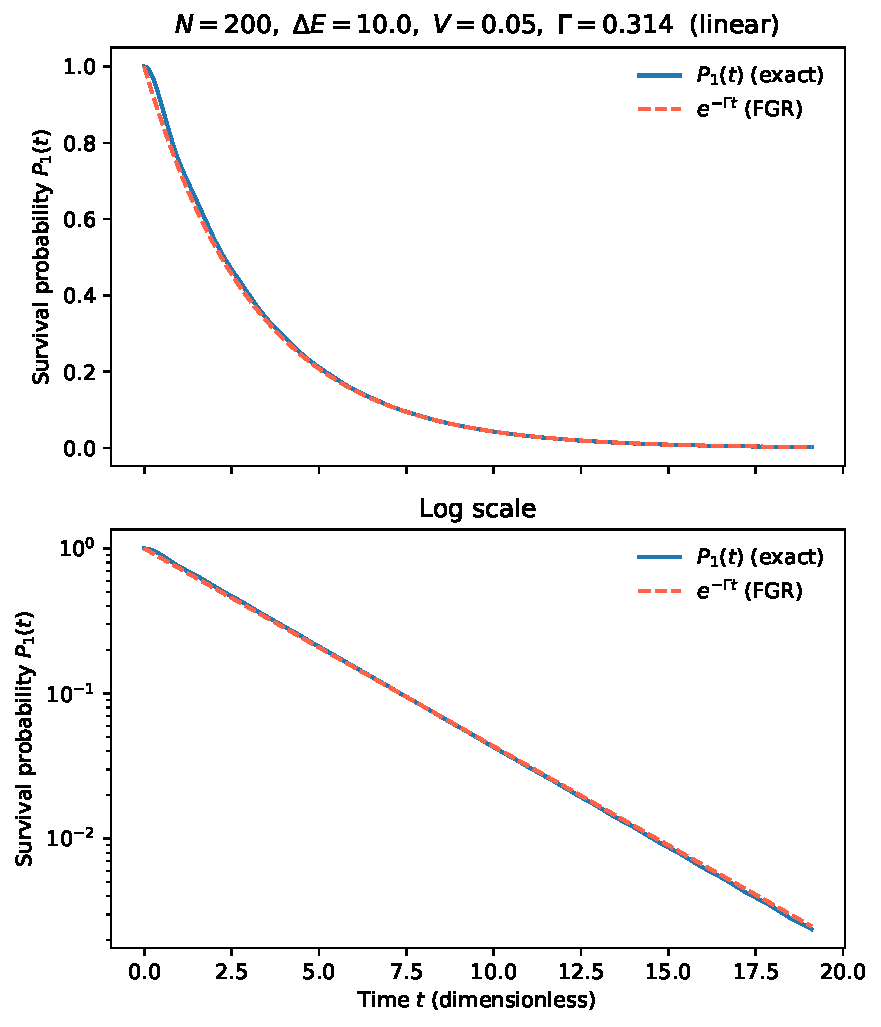
\includegraphics[width=\linewidth]{Model_A/Baseline/figures/Figure_baseline.pdf}
    \caption{Baseline dynamics of Model~A with $N=200$, $\Delta E=10$,
    $V_{1k}=0.05$, $E_1=0$ (dimensionless units, $\hbar=1$).
    The density of states is $\rho=20$, giving a FGR decay rate
    $\Gamma=2\pi V_{1k}^2\rho\approx 0.314$.
    Top: survival probability $P_1(t)$ (solid blue) versus the FGR
    prediction $e^{-\Gamma t}$ (dashed red) on a linear scale.
    Bottom: same data on a logarithmic scale, highlighting agreement
    over more than six orders of magnitude.
    The exact and FGR curves are virtually indistinguishable throughout
    the window $t\in[0,20]$, demonstrating quantitative validity of the
    wide-band approximation when $\rho^{-1}\ll\Gamma\ll\Delta E$.}
    \label{fig:baseline}
\end{figure}

\subsubsection{Effect of $N$}

To isolate the role of the bath discreteness from a change in the decay
rate, we define the \emph{reorganization energy}
\begin{equation}
    \Lambda \equiv \sum_{k=1}^{N}|V_{1k}|^2.
    \label{eq:hybridization}
\end{equation}
In the terminology of the present finite-level model, $\Lambda$ is simply
the total squared doorway--bath coupling strength.  It should not be
confused with the reorganization energy of shifted harmonic-oscillator
models, where the same phrase refers to an energy associated with equilibrium
coordinate displacements of explicit vibrational modes.
For the uniform-coupling case used here, $V_{1k}=V_N$ for all $k$, so
\begin{equation}
    \Lambda = N V_N^2.
    \label{eq:hybridization_uniform}
\end{equation}
We then rescale the coupling as
$V_N = V_{\mathrm{ref}}\sqrt{N_{\mathrm{ref}}/N}$ so that
\begin{equation}
    \Lambda = N V_N^2 = N_{\mathrm{ref}}V_{\mathrm{ref}}^2 = \mathrm{const}.
    \label{eq:hybridization_fixed}
\end{equation}
At fixed bandwidth $\Delta E$, this also fixes the FGR rate because
$\rho_N=N/\Delta E$ and therefore
\begin{equation}
    \Gamma = 2\pi V_N^2\rho_N = \frac{2\pi \Lambda}{\Delta E}.
    \label{eq:Gamma_hybridization}
\end{equation}
Thus varying $N$ at fixed $\Lambda$ changes only the bath discreteness and
the recurrence time, not the continuum-limit decay rate.  For the present
parameters, $\Lambda = 0.5$ and $\Gamma\approx 0.314$ for all $N$.
The Poincar\'e recurrence time
\begin{equation}
    T_{\mathrm{rec}} = \frac{2\pi}{\Delta\omega} = \frac{2\pi(N-1)}{\Delta E},
    \label{eq:Trec}
\end{equation}
where $\Delta\omega = \Delta E/(N-1)$ is the uniform level spacing, grows
linearly with $N$ at fixed $\Delta E$.

Figure~\ref{fig:effectN} compares $P_1(t)$ for $N=50$, $100$, and $200$
(with $V_N = 0.100$, $0.071$, and $0.050$, respectively) over a time window
extending beyond the longest $T_{\mathrm{rec}}$.
For all three cases the initial decay follows the common FGR exponential
$e^{-\Gamma t}$ closely, but a sharp Poincar\'e revival restores
substantial population to $\ket{1}$ at $t\approx T_{\mathrm{rec}}$
(annotated with arrows in the figure).
The revival is most prominent for small $N$: at $N=50$
($T_{\mathrm{rec}}\approx 30.8$) the peak revival amplitude exceeds $0.8$,
while at $N=200$ ($T_{\mathrm{rec}}\approx 125.0$) the revival occurs
far outside the experimentally relevant time window and the exponential
approximation is valid over many more decay lengths.
On the logarithmic scale the depth of the trough before the revival
deepens with increasing $N$, reflecting the improved continuum-limit
approximation.

\begin{figure}[htbp]
    \centering
    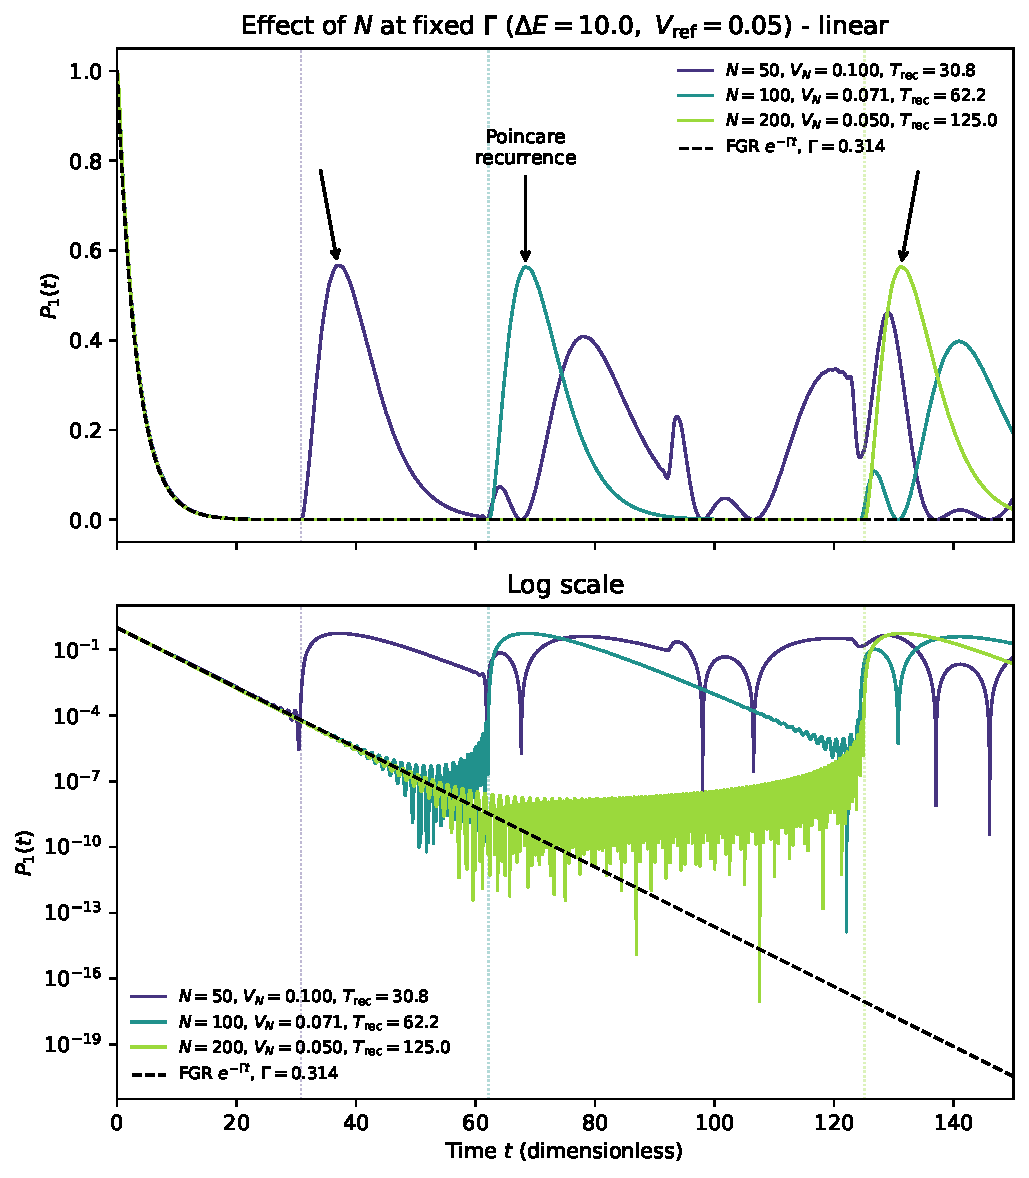
\includegraphics[width=\linewidth]{Model_A/Effect_of_N/figures/Figure_effect_N.pdf}
    \caption{Effect of the number of bath levels $N$ on the survival
    probability $P_1(t)$ of Model~A.
    The coupling is rescaled as $V_N = V_{\mathrm{ref}}\sqrt{N_{\mathrm{ref}}/N}$
    with $V_{\mathrm{ref}}=0.05$ and $N_{\mathrm{ref}}=200$, keeping the
    reorganization energy $\Lambda = NV_N^2 = 0.5$ and hence the FGR rate fixed at
    $\Gamma\approx 0.314$ for all curves.
    Parameters: $\Delta E=10$, $E_1=0$.
    Three bath sizes are shown: $N=50$ ($V_N=0.100$, $T_{\mathrm{rec}}\approx 30.8$,
    dark blue), $N=100$ ($V_N=0.071$, $T_{\mathrm{rec}}\approx 62.2$, teal), and
    $N=200$ ($V_N=0.050$, $T_{\mathrm{rec}}\approx 125.0$, yellow-green).
    The black dashed line is the FGR prediction $e^{-\Gamma t}$.
    Dotted vertical lines and arrows mark the Poincar\'e recurrence time
    $T_{\mathrm{rec}}$ for each $N$.
    Top: linear scale; bottom: logarithmic scale.
    All curves decay exponentially at rate $\Gamma$ before the first revival,
    demonstrating that exponential decay is an intermediate-time approximation
    valid only for $t\ll T_{\mathrm{rec}}$.}
    \label{fig:effectN}
\end{figure}

\subsubsection{Effect of $\Delta E$}

At fixed $N=200$ and $V_{1k}=0.05$, varying $\Delta E$ simultaneously
changes both the density of states $\rho=N/\Delta E$ and the ratio
$\Gamma/\Delta E = 2\pi V_{1k}^2 N/\Delta E^2$, which controls how well
the wide-band approximation is satisfied.
Figure~\ref{fig:effectDeltaE} shows $P_1(t)$ for four bandwidths
$\Delta E \in \{2,\,5,\,10,\,20\}$, corresponding to FGR rates
$\Gamma \approx \{1.57,\,0.63,\,0.31,\,0.16\}$ and ratios
$\Gamma/\Delta E \approx \{0.79,\,0.13,\,0.03,\,0.008\}$.

For the two widest bandwidths ($\Delta E = 10$ and $20$) the ratio
$\Gamma/\Delta E \ll 1$ and the dynamics are cleanly exponential, with
$P_1(t)$ indistinguishable from the respective FGR prediction.
As $\Delta E$ narrows, $\Gamma/\Delta E$ grows and the wide-band approximation
begins to fail: strong oscillations are already evident at $\Delta E = 2$,
the narrowest bandwidth shown, where $\Gamma/\Delta E \approx 0.79$ and the
doorway state is strongly influenced by the nearby band edges.
This onset of non-Markovian behavior is characterized by pronounced
oscillations throughout the observation window.
Conversely, larger $\Delta E$ pushes the band edges further from $E_1$
and deepens the Markovian limit, suppressing both oscillations and revivals.

\begin{figure}[htbp]
    \centering
    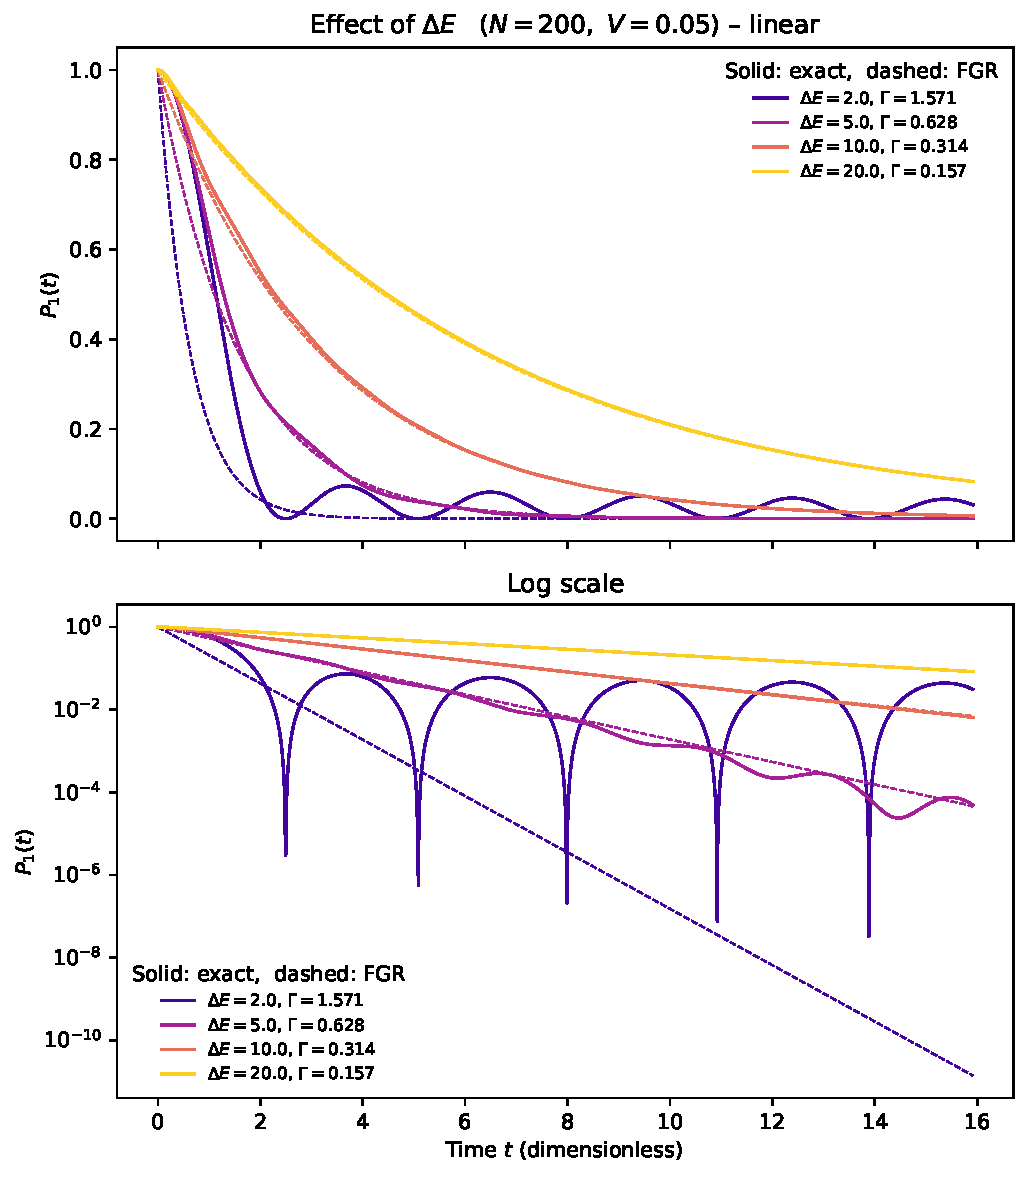
\includegraphics[width=\linewidth]{Model_A/Effect_of_DeltaE/figures/Figure_effect_DeltaE.pdf}
    \caption{Effect of the bath bandwidth $\Delta E$ on the survival
    probability $P_1(t)$ of Model~A with $N=200$, $V_{1k}=0.05$, $E_1=0$.
    Four values are shown: $\Delta E=2$ (magenta, $\Gamma\approx 1.57$),
    $\Delta E=5$ (blue, $\Gamma\approx 0.63$),
    $\Delta E=10$ (red, $\Gamma\approx 0.31$),
    $\Delta E=20$ (yellow, $\Gamma\approx 0.16$).
    The black dashed line is the FGR prediction for $\Delta E=10$.
    Top: linear scale; bottom: logarithmic scale.
    The narrowest bandwidth shown ($\Delta E=2$, $\Gamma/\Delta E\approx 0.8$)
    already violates the wide-band approximation and exhibits strongly
    non-exponential, oscillatory dynamics.
    Wider bandwidths ($\Delta E\geq 10$, $\Gamma/\Delta E\leq 0.03$) satisfy
    the approximation and recover clean exponential decay.}
    \label{fig:effectDeltaE}
\end{figure}

\subsubsection{Effect of $V_{1k}$}

Increasing $V_{1k}$ at fixed $N=200$ and $\Delta E=10$ raises $\Gamma$
through $\Gamma=2\pi V_{1k}^2\rho$, accelerating the decay while also
widening the resonance relative to the bath bandwidth.
Figure~\ref{fig:effectV} compares three coupling strengths
$V_{1k}\in\{0.05,\,0.1,\,0.15\}$, corresponding to
$\Gamma\approx\{0.314,\,1.257,\,2.827\}$ and
$\Gamma/\Delta E\approx\{0.03,\,0.13,\,0.28\}$.

For the weakest coupling ($V_{1k}=0.05$, $\Gamma/\Delta E\approx 0.03$)
the exact curve tracks the FGR exponential essentially perfectly over
the entire window.
At $V_{1k}=0.1$ ($\Gamma/\Delta E\approx 0.13$) the initial decay is
slightly faster than predicted by FGR and mild oscillations appear at later
times, signaling incipient breakdown of the wide-band approximation.
At $V_{1k}=0.15$ ($\Gamma/\Delta E\approx 0.28$) the departure is
substantial: the exact decay is markedly faster than $e^{-\Gamma t}$ at
early times and persistent Rabi-like oscillations dominate the long-time
dynamics, reflecting coherent coupling to the collective band mode.
These results confirm that the validity of FGR requires $\Gamma\ll\Delta E$,
not merely $\Gamma<\Delta E$.

\begin{figure}[htbp]
    \centering
    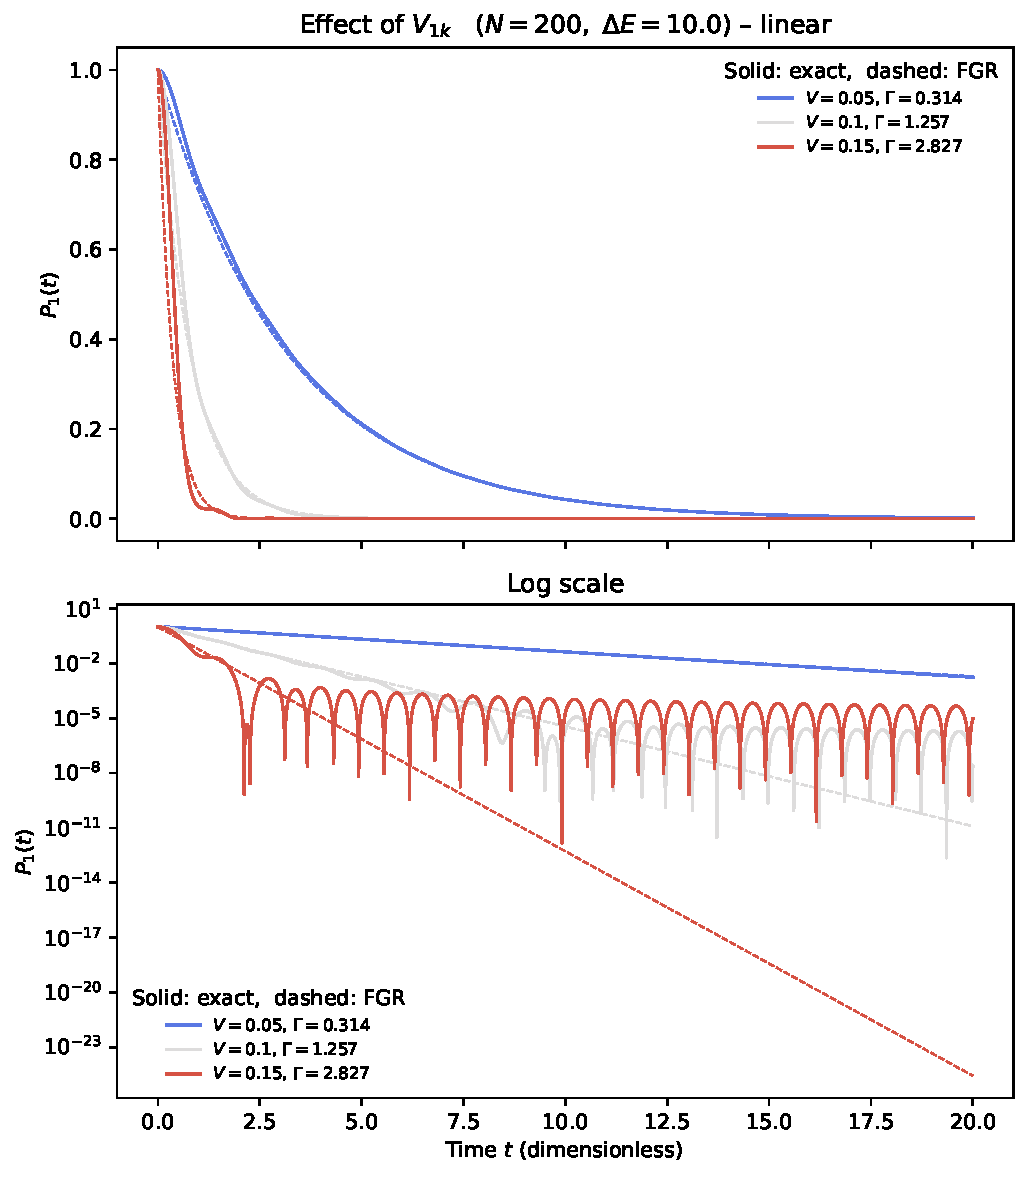
\includegraphics[width=\linewidth]{Model_A/Effect_of_V/figures/Figure_effect_V.pdf}
    \caption{Effect of the coupling strength $V_{1k}$ on the survival
    probability $P_1(t)$ of Model~A with $N=200$, $\Delta E=10$, $E_1=0$.
    Three values are shown: $V_{1k}=0.05$ (blue, $\Gamma\approx 0.314$,
    $\Gamma/\Delta E\approx 0.03$), $V_{1k}=0.10$ (silver/gray,
    $\Gamma\approx 1.257$, $\Gamma/\Delta E\approx 0.13$), and
    $V_{1k}=0.15$ (red, $\Gamma\approx 2.827$,
    $\Gamma/\Delta E\approx 0.28$).
    Solid lines are exact TDSE results; dashed lines of matching colour are
    the corresponding FGR predictions $e^{-\Gamma t}$.
    Top: linear scale; bottom: logarithmic scale, $t\in[0,20]$.
    As $V_{1k}$ increases the resonance width $\Gamma$ approaches the
    bandwidth $\Delta E$, causing the exact decay to deviate progressively
    from the FGR exponential and eventually to exhibit sustained oscillations
    (crossover from Markovian-looking decay to coherent oscillatory dynamics).}
    \label{fig:effectV}
\end{figure}

\subsubsection{Uniform versus random-sign couplings}

For Model~A, replacing uniform couplings $V_{1k}=V$ with equal-magnitude
random-sign couplings $V_{1k}=\pm V$ leaves the survival probability
$P_1(t)$ \emph{unchanged}.  This is a structural consequence of the
Hamiltonian topology: since each manifold state $\ket{k}$ couples only to
the single doorway state $\ket{1}$, the sign of $V_{1k}$ can be absorbed
into a redefinition $\ket{k}\to-\ket{k}$, which is a valid unitary
transformation that leaves all physical observables invariant.
Gaussian couplings
$V_{1k}\overset{\mathrm{i.i.d.}}{\sim}\mathcal{N}(0,V^2)$ introduce
seed-to-seed fluctuations, widening
the envelope of $P_1(t)$ while preserving the mean decay rate.

Figure~\ref{fig:couplingDisorder} shows $P_1(t)$ for all three coupling
schemes ($N=200$, $\Delta E=10$, $V_{\mathrm{rms}}=0.05$, averaged over
1000 disorder realisations with $\pm1\sigma$ shaded bands).
As expected, the uniform and random-sign curves are numerically identical.
The Gaussian ensemble mean also tracks the FGR prediction closely, but with
a visible spread reflecting magnitude disorder: realisations with larger
$\langle V_{1k}^2\rangle^{1/2}$ decay faster while those with smaller
values decay more slowly, smearing the revival structure.
All three schemes satisfy $\langle\Gamma\rangle = 2\pi V_{\mathrm{rms}}^2\rho$
to within statistical uncertainty.

\begin{figure}[htbp]
    \centering
    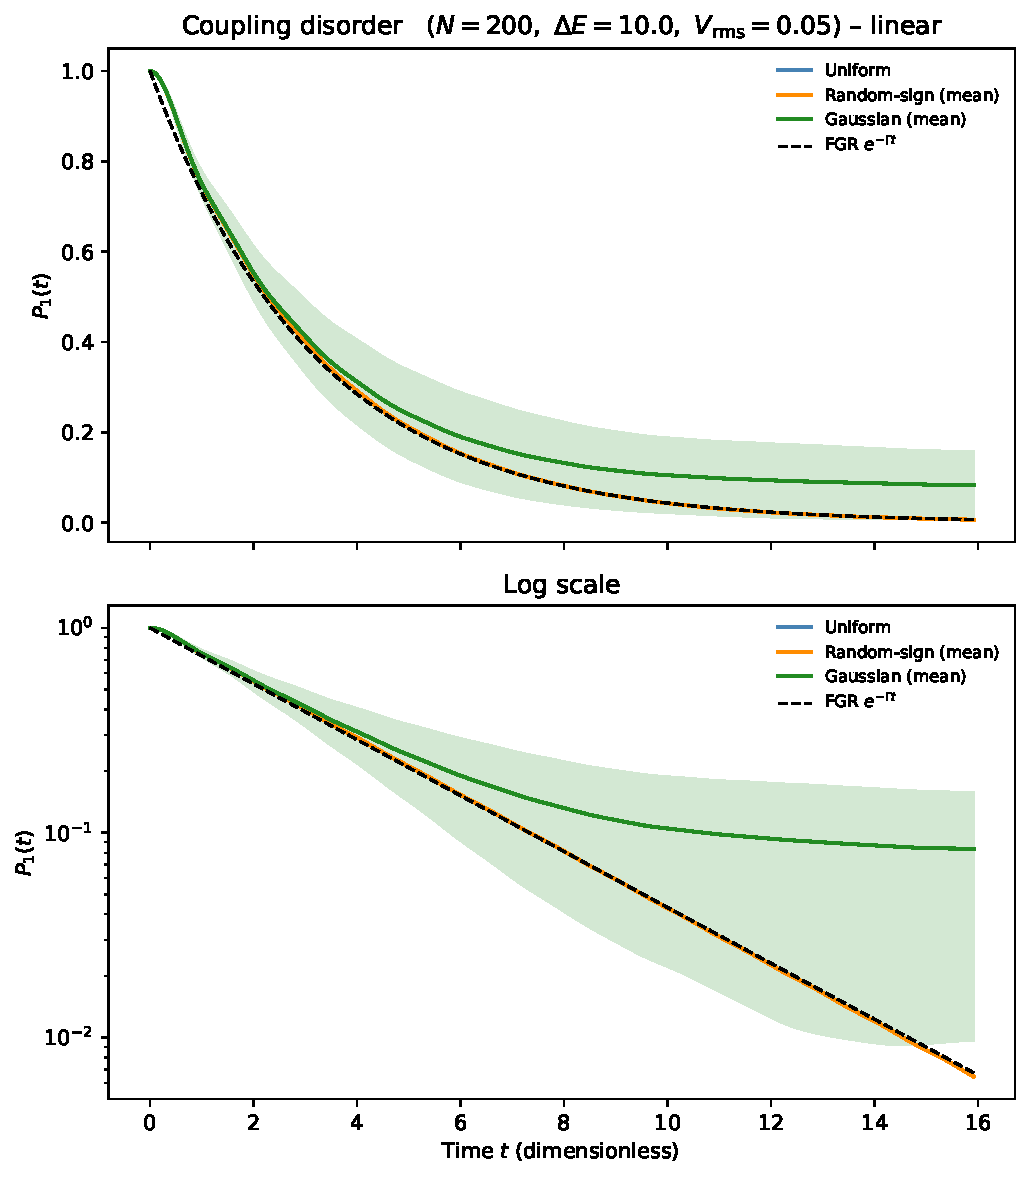
\includegraphics[width=\linewidth]{Model_A/Coupling_disorder/figures/Figure_coupling_disorder.pdf}
    \caption{Effect of coupling disorder on $P_1(t)$ in Model~A
    ($N=200$, $\Delta E=10$, $V_{\mathrm{rms}}=0.05$, $E_1=0$).
    Three coupling schemes are compared: uniform $V_{1k}=V$ (blue solid),
    random-sign $V_{1k}=\pm V$ (orange, mean over 1000 realisations), and
    Gaussian $V_{1k}\overset{\mathrm{i.i.d.}}{\sim}\mathcal{N}(0,V^2)$
    (green, mean over 1000 realisations).
    Shaded bands denote $\pm1$ standard deviation across realisations.
    The black dot-dashed line is the FGR prediction $e^{-\Gamma t}$ with
    $\Gamma=2\pi V^2\rho\approx 0.314$.
    Top: linear scale; bottom: logarithmic scale.
    Uniform and random-sign results are numerically identical due to a
    gauge equivalence (sign redefinition of bath states).
    The Gaussian ensemble reproduces the same mean decay rate but exhibits
    broader realization-to-realization variance, especially at late times.}
    \label{fig:couplingDisorder}
\end{figure}

\subsection{Model B: two-step relaxation dynamics}

\subsubsection{Sequential population flow}

\begin{figure*}[t]
  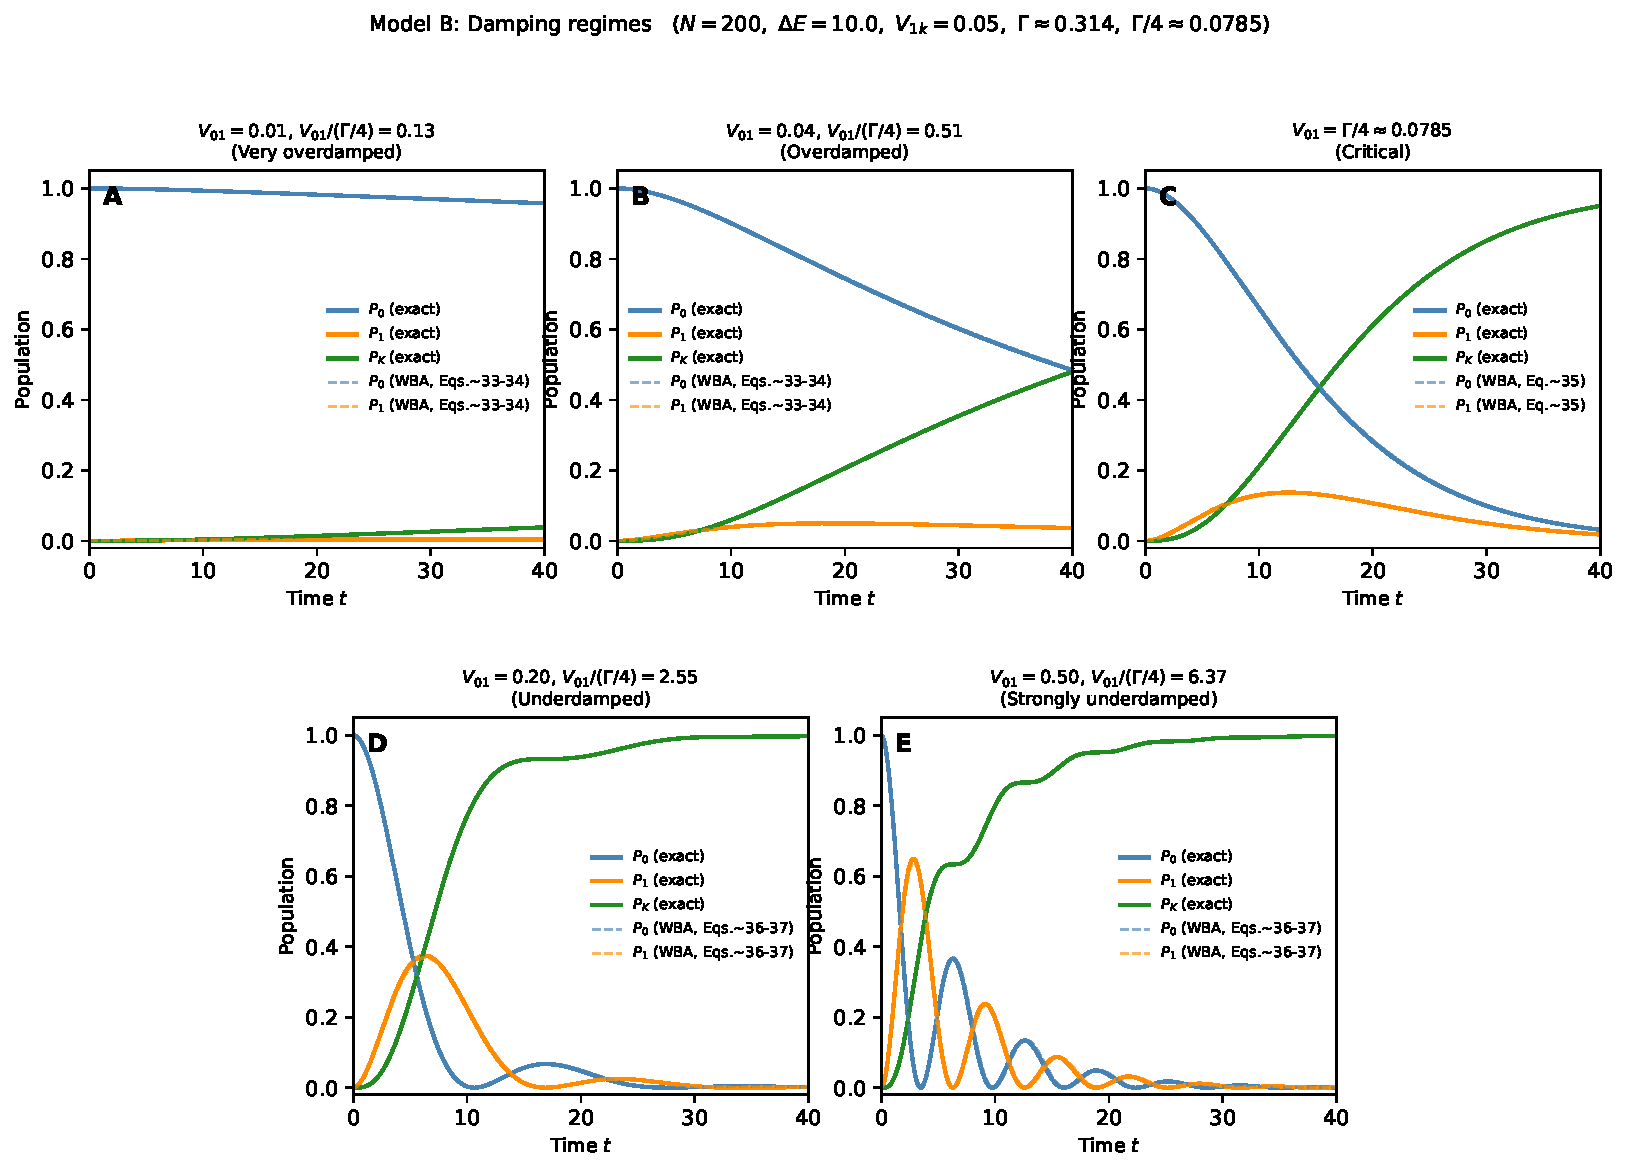
\includegraphics[width=\linewidth]{Model_B/Sequential_flow/figures/Figure_sequential_flow.pdf}
  \caption{\label{fig:seqFlow}%
    \textbf{Five damping regimes of Model~B}, classified by the ratio
    $V_{01}/(\Gamma/4)$ (Sec.~\ref{sec:GF}).
    Parameters: $N=200$, $\Delta E=10$, $V_{1k}=0.05$, $E_0=E_1=0$,
    $\Gamma\approx0.314$, $\Gamma/4\approx0.0785$; $t_{\max}=40$.
    Solid lines: exact TDSE. Dashed lines: WBA analytical solution
    from Sec.~\ref{sec:GF}, based on Eqs.~\ref{eq:damped_c0}
    and \ref{eq:lambdaB}.
    Blue: $P_0(t)$; orange: $P_1(t)$; green: $P_K(t)=1-P_0-P_1$.
    Upper row (A--C): overdamped side of the transition.
    \textbf{(A)} $V_{01}=0.01$ ($V_{01}/(\Gamma/4)=0.13$, very overdamped):
    $P_0$ barely decays over the window;
    $\gamma_{\rm eff}=2V_{01}^{2}/\Gamma\approx6.4\times10^{-4}$.
    \textbf{(B)} $V_{01}=0.04$ ($V_{01}/(\Gamma/4)=0.51$, overdamped):
    monotonic decay with $\gamma_{\rm eff}\approx0.010$.
    \textbf{(C)} $V_{01}=\Gamma/4\approx0.0785$ (critical): fastest
    non-oscillatory transfer; $P_1$ transient is maximal.
    Lower row (D--E): underdamped side.
    \textbf{(D)} $V_{01}=0.20$ ($V_{01}/(\Gamma/4)=2.55$): several
    damped Rabi cycles with $2\Omega_{\rm u}\approx0.37$.
    \textbf{(E)} $V_{01}=0.50$ ($V_{01}/(\Gamma/4)=6.37$): rapid coherent
    oscillations ($2\Omega_{\rm u}\approx0.99$, period $\approx 6.3$)
    with full damping envelope $e^{-\Gamma t/4}$ within the window.
    WBA dashed lines agree with the exact TDSE in all panels.}
\end{figure*}

In Model~B the population must flow from $\ket{0}$ to $\ket{1}$ before it
can relax into the bath manifold.  As derived in Sec.~\ref{sec:GF},
integrating out the bath in the wide-band limit reduces the $\ket{0}$--$\ket{1}$
subspace to a damped two-level problem; on resonance, the amplitude
$c_0(t)$ satisfies the same second-order equation as a damped harmonic
oscillator [Eq.~\eqref{eq:damped_c0}], with the bath setting $\Gamma$
and $V_{01}$ playing the role of the restoring frequency.
The critical threshold is $V_{01}=\Gamma/4\approx0.0785$.
Figure~\ref{fig:seqFlow} surveys five representative values of $V_{01}$
at fixed $N=200$, $\Delta E=10$, $V_{1k}=0.05$ ($\Gamma\approx0.314$),
$E_0=E_1=0$, and $t_{\max}=40$, spanning the full range from very
overdamped to strongly underdamped dynamics.

Panels~A and~B show two overdamped cases.
At $V_{01}=0.01$ (panel~A, $V_{01}/(\Gamma/4)=0.13$), the system is
deeply overdamped: the effective rate $\gamma_{\rm eff}=2V_{01}^{2}/\Gamma
\approx6.4\times10^{-4}$ is so small that $P_0$ remains near unity
over the entire window, $P_1$ is a barely visible transient, and $P_K$
stays essentially zero.  Increasing to $V_{01}=0.04$ (panel~B,
$V_{01}/(\Gamma/4)=0.51$) accelerates the decay to
$\gamma_{\rm eff}\approx0.010$; $P_0$ falls noticeably and a small
$P_1$ transient develops, but the dynamics remains monotonic.

Panel~C shows critical damping ($V_{01}=\Gamma/4\approx0.0785$), the
boundary between regimes.  The characteristic exponents $\lambda_{\pm}$
are degenerate, giving the $P_0$ envelope $e^{-\Gamma t/4}(1+\Gamma t/4)$.
Population reaches the bath as quickly as possible without oscillating,
and the $P_1$ transient is larger than in either overdamped panel.

Panels~D and~E exhibit underdamped coherent dynamics.
At $V_{01}=0.20$ (panel~D, $V_{01}/(\Gamma/4)=2.55$), damped Rabi
oscillations with frequency $2\Omega_{\rm u}=
2\sqrt{V_{01}^{2}-(\Gamma/4)^{2}}\approx0.37$ are clearly resolved;
$P_K$ rises in a staircase pattern that mirrors each half-cycle of
population transfer.  At $V_{01}=0.50$ (panel~E,
$V_{01}/(\Gamma/4)=6.37$), the oscillation frequency
$2\Omega_{\rm u}\approx0.99$ is large enough that roughly six full
Rabi cycles are completed before the $e^{-\Gamma t/4}$ envelope
damps the amplitude to zero, with $P_K$ filling entirely within the
window.  In all five panels the WBA analytical prediction (dashed)
agrees quantitatively with the exact TDSE result, validating the
wide-band approximation across the full parameter range.

\subsubsection{Effect of $E_0 - E_1$}

\begin{figure*}[htbp]
  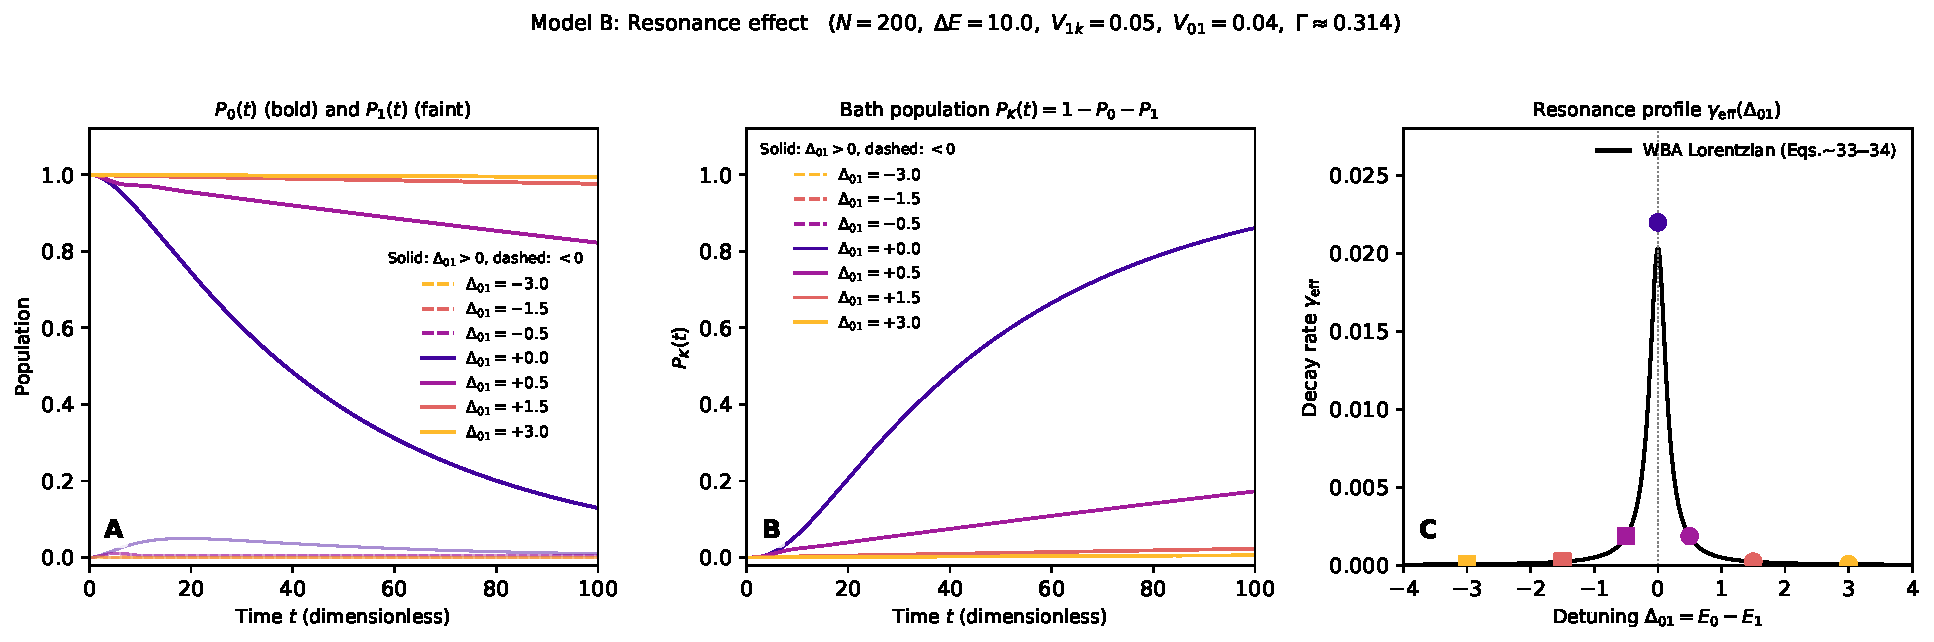
\includegraphics[width=\linewidth]{Model_B/Effect_of_E0_E1/figures/Figure_effect_E0_E1.pdf}
  \caption{\label{fig:resonance}%
    \textbf{Resonance effect in Model~B.}
    Parameters: $N=200$, $\Delta E=10$, $V_{1k}=0.05$, $V_{01}=0.04$
    (overdamped, panel~B of Fig.~\ref{fig:seqFlow}), $\Gamma\approx0.314$;
    $t_{\max}=100$.
    Detunings $\Delta_{01}\in\{0,\pm0.5,\pm1.5,\pm3.0\}$; solid lines:
    $\Delta_{01}>0$, dashed: $\Delta_{01}<0$; same color for $\pm|\Delta_{01}|$.
    \textbf{(A)} Both $P_0(t)$ (bold) and $P_1(t)$ (faint, same color):
    $P_0$ decays fastest at resonance ($\Delta_{01}=0$) while $P_1$ builds
    up to its largest transient; both are progressively suppressed as
    $|\Delta_{01}|$ grows.
    \textbf{(B)} Bath population $P_K(t)=1-P_0-P_1$: $P_K$ fills up
    rapidly at resonance and saturates near unity, while off-resonance
    population remains trapped in $\ket{0}$ over the window.
    Positive and negative detunings give identical dynamics, confirming
    the energy-reflection symmetry of the bath.
    \textbf{(C)} Extracted population decay rate $\gamma_\mathrm{eff}$ versus
    $\Delta_{01}$ (circles: $\Delta_{01}>0$; squares: $\Delta_{01}<0$),
    overlaid with the WBA Lorentzian
    $\gamma_\mathrm{eff}=V_{01}^{2}\Gamma/(\Delta_{01}^{2}+(\Gamma/2)^{2})$
    (black curve).  The Lorentzian has width $\Gamma/2\approx0.157$ and
    peak $4V_{01}^{2}/\Gamma\approx0.020$.}
\end{figure*}

The energy offset $\Delta_{01}=E_0-E_1$ controls how efficiently population
can flow from $\ket{0}$ to $\ket{1}$.  Using the overdamped parameter $V_{01}=0.04$
(panel~B of Fig.~\ref{fig:seqFlow}), Fig.~\ref{fig:resonance} scans
$\Delta_{01}\in\{0,\pm0.5,\pm1.5,\pm3.0\}$ with $t_{\max}=100$, long enough
to resolve the slow resonant decay $\gamma_0=4V_{01}^{2}/\Gamma\approx0.020$.

At $\Delta_{01}=0$ (resonance), $P_0$ decays at the maximum rate, $P_1$
builds up to its largest transient (panel~A), and $P_K$ fills up rapidly
to near unity (panel~B).  As $|\Delta_{01}|$ increases, the
effective transfer rate drops sharply: at $|\Delta_{01}|=0.5$ it falls
to $\approx9\%$ of the resonant value, and at $|\Delta_{01}|=3.0$ to
below $0.3\%$.  This rapid suppression is captured by the Lorentzian
(panel~C), whose half-width at half-maximum is the bath-induced linewidth
$\Gamma/2\approx0.157$, far smaller than the bath bandwidth $\Delta E/2=5$.

A key observation is that positive and negative detunings produce
\emph{identical} $P_0(t)$ and $P_1(t)$ curves (solid and dashed lines
overlap exactly in panels~A and~B).  This follows from the energy-reflection
symmetry of the model: the bath spectrum is symmetric about $E_1=0$, so
$\Delta_{01}\to-\Delta_{01}$ is equivalent to reversing all energies,
which leaves populations unchanged.

The effective decay rate plotted in panel~C is extracted from the TDSE data
as follows.  In the overdamped regime the fast normal mode of $H_\mathrm{eff}$
decays on the timescale $\sim 1/\Gamma \approx 3$, leaving a single
slow exponential $P_0(t)\approx A\,e^{-\gamma_\mathrm{eff}t}$ for $t \gg 1/\Gamma$.
We therefore fit $\ln P_0(t)$ to a straight line over the second half of
the simulation window ($t\in[50,100]$), where the fast transient has fully
died out and $P_0$ is still well above numerical noise.
The slope of the linear fit gives $\gamma_\mathrm{eff}$ directly.
This procedure is reliable provided $P_0$ has not yet been fully depleted,
which is satisfied for all detunings shown ($P_0(100)\gtrsim10^{-2}$ even
at resonance).

Panel~C demonstrates that the WBA Lorentzian prediction agrees quantitatively
with the numerically extracted rates across the full scan, confirming that
the Breit--Wigner line shape governs the resonance structure of the two-step
decay process.

\subsubsection{Effect of $N$ in Model B}

\begin{figure*}[htbp]
  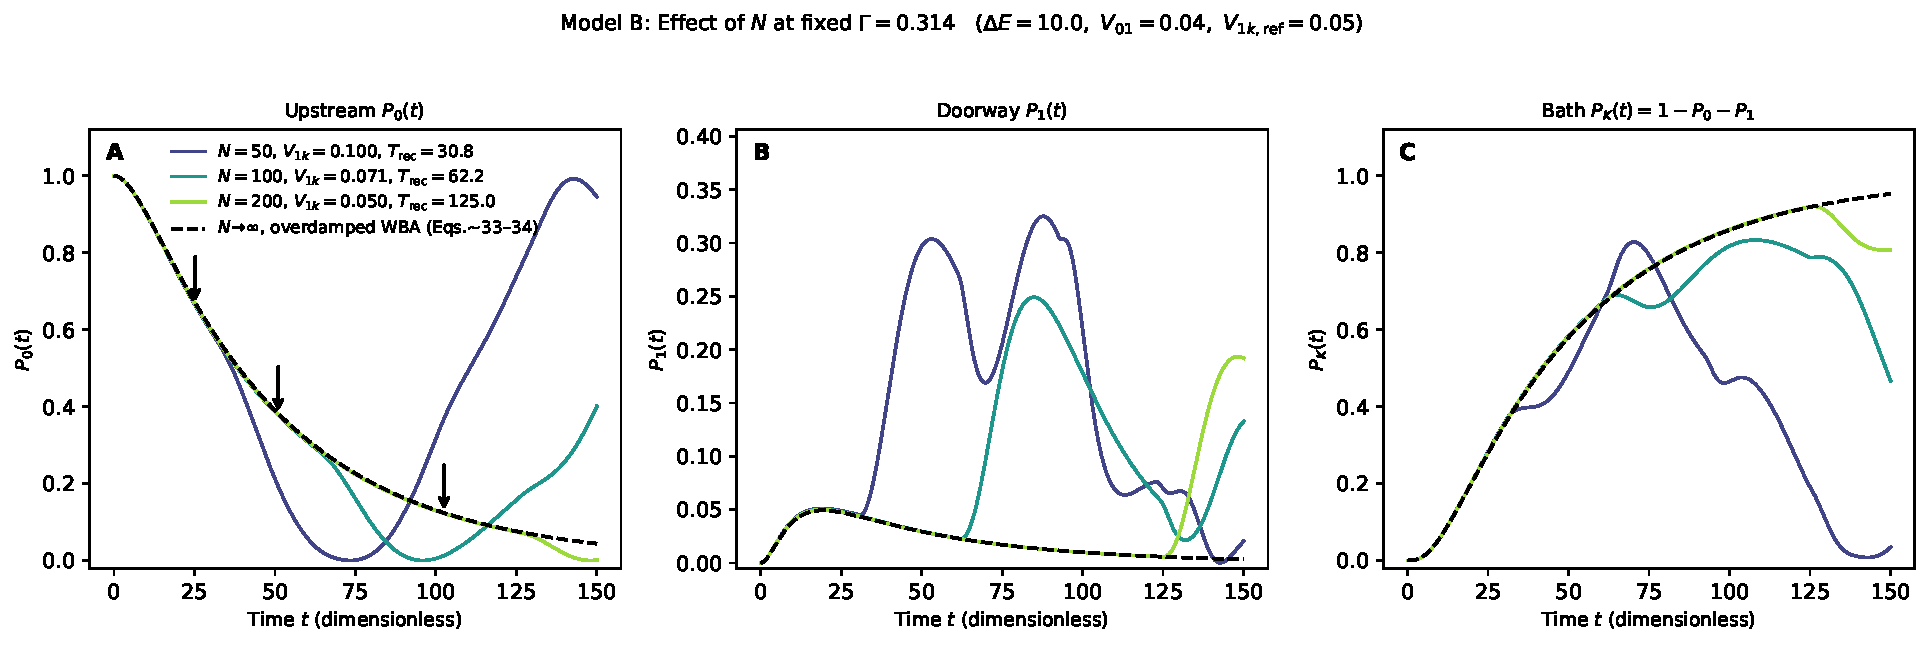
\includegraphics[width=\linewidth]{Model_B/Effect_of_N/figures/Figure_effect_N_modelB.pdf}
  \caption{\label{fig:effectNB}%
    \textbf{Effect of bath size $N$ in Model~B at fixed reorganization energy.}
    Following the design of Fig.~\ref{fig:effectN}, $V_{1k}$ is scaled as
    $V_{1k}(N)=V_{\rm ref}\sqrt{N_{\rm ref}/N}$ with $V_{\rm ref}=0.05$,
    $N_{\rm ref}=200$ so that $\Lambda = NV_{1k}^{2}=0.5$ and
    $\Gamma\approx0.314$ are held constant.
    The upstream coupling is fixed at $V_{01}=0.04$ (overdamped,
    same as Fig.~\ref{fig:resonance}); $\Delta E=10$, $E_0=E_1=0$.
    Parameter values: $N=50$ ($V_{1k}=0.100$, $T_{\rm rec}=30.8$),
    $N=100$ ($V_{1k}=0.071$, $T_{\rm rec}=62.2$),
    $N=200$ ($V_{1k}=0.050$, $T_{\rm rec}=125.0$).
    Black dashed line: $N\!\to\!\infty$ WBA analytical result
    from Sec.~\ref{sec:GF}.
    Black downward arrows point to the Poincar\'e revival feature
    (local maximum in $P_0$, $P_1$; local minimum in $P_K$) for each $N$.
    \textbf{(A)} Upstream population $P_0(t)$: all three finite-$N$ curves
    nearly coincide with the WBA limit, confirming that $P_0$ is
    rate-limited by $V_{01}$, not $N$.  Revival bumps visible at each
    $T_{\rm rec}$ as population briefly returns from the bath.
    \textbf{(B)} Doorway population $P_1(t)$: revival peaks at $T_{\rm rec}$
    grow in prominence as $N$ decreases (shorter recurrence time).
    \textbf{(C)} Bath population $P_K(t)=1-P_0-P_1$: all curves fill at the
    same rate; brief dips at $T_{\rm rec}$ coincide with the revivals in
    panels~A and~B.}
\end{figure*}

Figure~\ref{fig:effectNB} compares $N=50$, $100$, $200$ with $V_{1k}$
scaled to keep $\Gamma\approx0.314$ and $\Lambda = NV_{1k}^{2}=0.5$ fixed, and
with $V_{01}=0.04$ (overdamped, same parameter regime as Fig.~\ref{fig:resonance}).
The black dashed line shows the $N\!\to\!\infty$ WBA analytical result from
Sec.~\ref{sec:GF}: in this limit the bath is a true continuum and no Poincar\'e
revival occurs, so $P_0$, $P_1$, $P_K$ vary smoothly for all time.
The three $P_0(t)$ curves in panel~A are nearly superimposed and closely
track the WBA prediction, confirming that the rate-limiting step is the
$\ket{0}\!\to\!\ket{1}$ coupling, which depends only on $V_{01}$ and is
independent of the bath density of states.
Panel~B shows that the doorway state $P_1(t)$ carries a small transient
determined by $V_{01}$ and $\Gamma$; small revivals appear at each
$T_{\rm rec}$ as population briefly returns from the bath to $\ket{1}$.
Panel~C confirms that $P_K$ fills identically for all $N$ on the initial
decay, with brief dips at $T_{\rm rec}$ corresponding to the Poincar\'e
recurrence: the discrete bath returns its population to the system before
it re-enters the bath manifold.  The revival amplitude is smaller than in
Model~A (Fig.~\ref{fig:effectN}) because population must traverse the extra
$\ket{1}\!\to\!\ket{0}$ step to reach $P_0$, attenuating the recurrence
signal.  Larger $N$ pushes $T_{\rm rec}$ to longer times, extending the
window over which the Markovian exponential approximation is valid.

\subsubsection{Coupling disorder in Model B}

\begin{figure*}[htbp]
  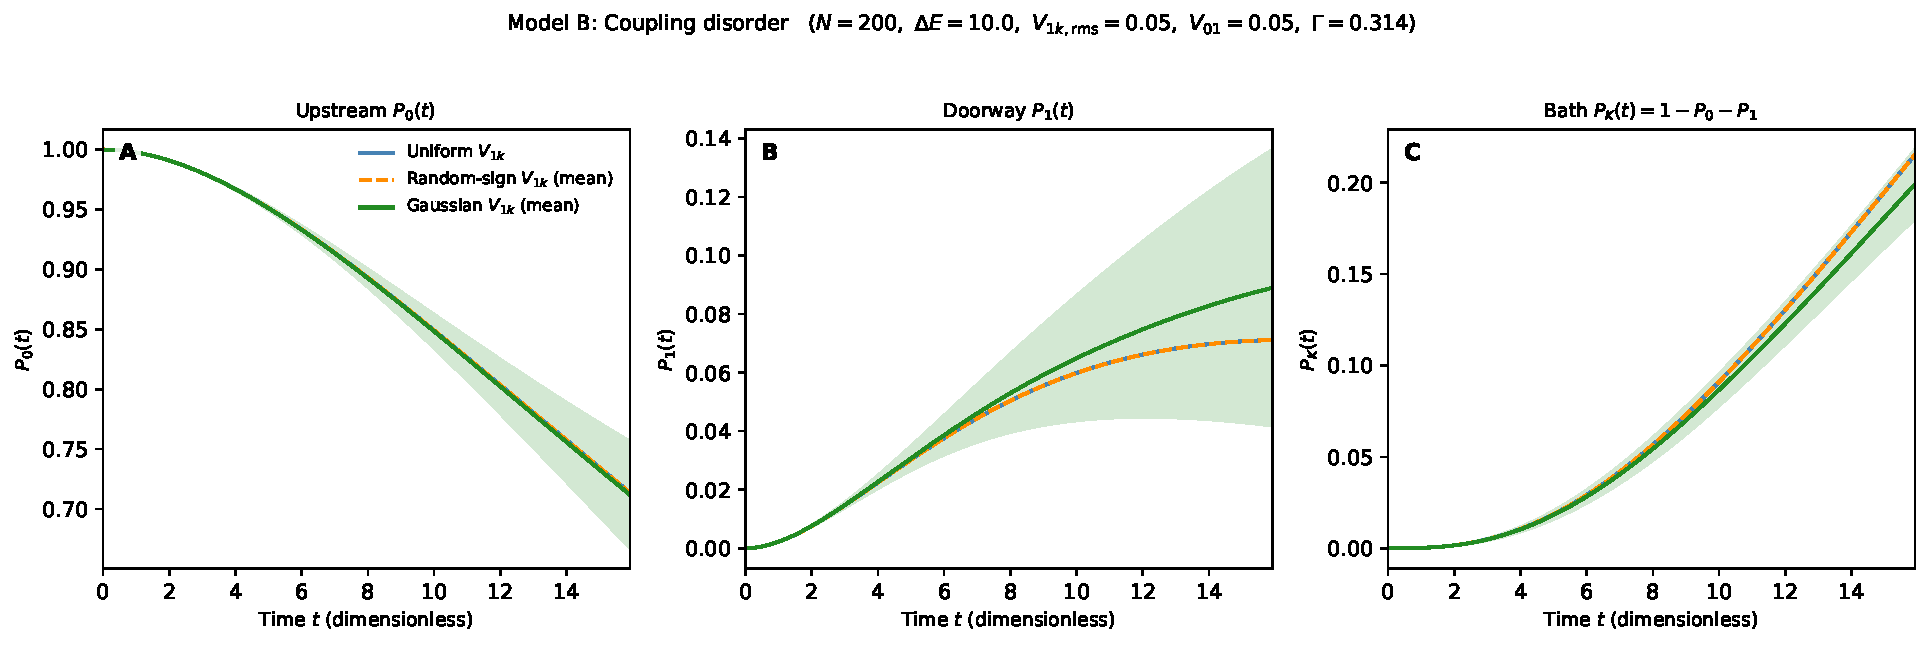
\includegraphics[width=\linewidth]{Model_B/Coupling_disorder/figures/Figure_coupling_disorder_modelB.pdf}
  \caption{\label{fig:disorderB}%
    \textbf{Effect of coupling disorder in Model~B.}
    Parameters: $N=200$, $\Delta E=10$, $V_{1k,\rm rms}=0.05$, $V_{01}=0.05$,
    $\Gamma=0.314$; ensemble of 1000 realisations for stochastic cases.
    Shaded bands show $\pm1$ standard deviation over realisations.
    Panel~A: upstream population $P_0(t)$.
    Panel~B: doorway population $P_1(t)$.
    Panel~C: bath population $P_K(t)=1-P_0-P_1$.
    \emph{Blue (uniform $V_{1k}$):} deterministic baseline.
    \emph{Orange dashed (random-sign $V_{1k}$):} mean coincides with the uniform
    curve and the band collapses to zero, confirming the gauge equivalence
    that extends from Model~A to Model~B when $V_{01}$ is fixed.
    \emph{Green (Gaussian $V_{1k}$):} genuine disorder shifts the mean and
    broadens $P_1(t)$ near its transient peak; the variance is reflected
    symmetrically in $P_K(t)$ while leaving the slower $P_0(t)$ decay
    comparatively unaffected.}
\end{figure*}

Figure~\ref{fig:disorderB} overlays three coupling schemes for Model~B
($N=200$, $\Delta E=10$, $V_{1k,\rm rms}=V_{01}=0.05$) across three panels
showing $P_0(t)$ (panel~A), $P_1(t)$ (panel~B), and the bath population
$P_K(t)=1-P_0-P_1$ (panel~C).

\emph{Random-sign $V_{1k}$} is again indistinguishable from the uniform
case.  As in Model~A, flipping the sign of an individual coupling
$V_{1k}\to -V_{1k}$ is a gauge transformation on bath state $\ket{k}$ that
leaves all populations unchanged, so the mean and the ensemble spread both
collapse onto the uniform baseline in all three panels.

\emph{Gaussian $V_{1k}$} introduces genuine disorder.  Averaged over 1000
realisations, $P_0(t)$ acquires a moderate but well-converged sample-to-sample
variance because different realisations carry different effective $\Gamma$;
the variance grows over the observation window.
$P_1(t)$ shows a larger relative variance near its transient peak: realisations
with stronger bath couplings drain $\ket{1}$ faster, producing an earlier and
smaller peak.  The bath population $P_K(t)$ mirrors the complementary
variance: when $P_0$ and $P_1$ fluctuate, the excess probability must reside
in the bath, so the spread in $P_K$ reflects the combined disorder from both
upstream states.

The sign of the upstream coupling $V_{01}$ is a global gauge freedom.  A
sign change $V_{01}\to -V_{01}$ is equivalent to $\ket{0}\to -\ket{0}$,
which shifts the phase of the initial amplitude without affecting any
population $|\braket{j|\psi(t)}|^{2}$.  Randomising the sign of $V_{01}$
therefore produces dynamics identical to the uniform case, and no disorder
effect is observable.

%-----------------------------------------------------------------------
\section{Conclusions}
%-----------------------------------------------------------------------

We have carried out a combined analytical and numerical study of quantum
relaxation in two finite-dimensional doorway-state models.  The principal
conclusions are as follows.

\begin{enumerate}
\item \textbf{Model~A: Green's-function theory and exponential decay.}
For a single doorway state coupled to a bath manifold, the retarded
Green's-function / self-energy treatment reproduces the Fermi's-golden-rule
result $P_1(t)=e^{-\Gamma t}$ under the wide-band approximation.  The exact
TDSE numerics confirm that this Markovian exponential regime is realized
when $\rho^{-1}\lesssim\Gamma\ll\Delta E$, and that the agreement improves
as the bath becomes denser and broader.

\item \textbf{Finite-size effects and breakdown of the wide-band regime.}
In a finite bath the exponential law is only an intermediate-time
approximation.  The recurrence time
$T_{\mathrm{rec}}\approx 2\pi N/\Delta E$ sets the onset of quantum
Poincar\'e recurrences, while small $\Delta E$, small $N$, or large $V_{1k}$
drive the system out of the wide-band limit and generate non-Markovian
oscillations.  Conversely, if $V_{1k}$ becomes too small compared with
$\rho^{-1}$, the manifold no longer behaves as a continuum and the FGR
picture also fails.

\item \textbf{Model~B: damped two-level dynamics under the wide-band approximation.}
When the bath coupled to $\ket{1}$ satisfies the same wide-band conditions,
Model~B reduces to an effective damped two-level system for the pair
$\{\ket{0},\ket{1}\}$ only because the doorway state is assumed, under the
wide-band approximation, to decay Markovianly at rate $\Gamma$.  The
analytical theory then predicts three regimes separated by
$V_{01}=\Gamma/4$: overdamped transfer for $V_{01}<\Gamma/4$, critical
damping at $V_{01}=\Gamma/4$, and damped Rabi oscillations for
$V_{01}>\Gamma/4$.  The exact TDSE calculations agree quantitatively with
this classification over the parameter range where the WBA is valid.

\item \textbf{Resonance structure in Model~B.}
The energy offset $\Delta_{01}=E_0-E_1$ acts as a detuning parameter for the
upstream-to-doorway transfer.  In the overdamped regime the effective decay
rate follows the Lorentzian form
$\gamma_{\mathrm{eff}}=V_{01}^{2}\Gamma/(\Delta_{01}^{2}+(\Gamma/2)^{2})$,
so population transfer is maximal at resonance and strongly suppressed for
large $|\Delta_{01}|$.  Positive and negative detunings give identical
dynamics due to the energy-reflection symmetry of the model.

\item \textbf{Effect of coupling disorder.}
Random-sign couplings are exactly gauge-equivalent to uniform couplings and
therefore leave all populations unchanged in both models.  By contrast,
Gaussian-distributed bath couplings introduce genuine disorder: the mean
dynamics remains close to the corresponding wide-band prediction, but
sample-to-sample fluctuations broaden the envelopes and are most visible in
the transient doorway population and in late-time recurrence features.
\end{enumerate}

Taken together, these results provide a unified picture of doorway-state
relaxation in finite systems.  The wide-band approximation is the bridge
from finite Hamiltonians to irreversible-looking decay, and the exact
numerics show where that bridge holds and where it fails.  More
fundamentally, irreversible relaxation is not an intrinsic property of a
finite quantum system, but an emergent continuum-limit phenomenon in which
phase randomization suppresses coherent recurrences over the timescale of
observation.

At the same time, the present study remains intentionally minimal: the bath
is represented by discrete levels, the analysis is effectively restricted to
zero-temperature relaxation, and no explicit molecular vibrational
coordinates are included.  These simplifications clarify the origin and
breakdown of the wide-band approximation, but they also limit direct
chemical realism.

Future work should embed the present doorway-state picture in more
microscopic open-system models.  In particular, replacing the discrete
phenomenological bath by an explicit oscillator environment, such as a
Caldeira--Leggett model~\cite{Caldeira_Leggett_1983,Leggett_1984,Weiss},
would allow temperature effects, spectral densities, memory kernels, and
vibronic structure to be treated on the same footing.  Even in their present
form, however, these models provide a useful minimal framework for
understanding relaxation in molecular systems, nanoscale devices, and open
quantum systems with structured environments.

%-----------------------------------------------------------------------
\section*{Data and code availability}
%-----------------------------------------------------------------------

The data and code that support the findings of this study are available at
\url{https://github.com/Okita0512/CHEM-5260-Midterm-Project}.

%-----------------------------------------------------------------------
\begin{acknowledgments}
The author thanks Prof.~Abraham Nitzan for designing this midterm project. The author also thanks the students of
CHEM~5260 (Spring 2026) whose numerical experiments informed and inspired
the analysis presented here. The author acknowledges Claude Code for
assistance in generating the Python scripts used for data production and
plotting, and ChatGPT for assistance with writing and revising this
document.
\end{acknowledgments}

%-----------------------------------------------------------------------
\bibliographystyle{apsrev4-2}
\bibliography{ref}

\end{document}
